%------------------------------ GENERALIDADES ----------------------------
%\chapter{CAPITULO 1}
\chapter{GENERALIDADES}
\section{Introducción}

En la actualidad, la incorporación de sistemas electrónicos en los vehículos ha permitido mejorar significativamente el control, diagnóstico y eficiencia en su funcionamiento. A través de diferentes sensores y unidades de control electrónico, es posible obtener información relevante sobre el desempeño del motor y otros subsistemas en tiempo real. En este contexto, el estándar OBD-II (On-Board Diagnostics) se ha consolidado como una herramienta fundamental para el acceso a datos vehiculares.

El presente proyecto tiene como finalidad el desarrollo de un sistema de monitoreo del consumo de combustible en vehículos que no disponen de esta funcionalidad de forma nativa. Si bien algunos vehículos modernos ya incorporan sistemas que permiten visualizar este tipo de información directamente en el panel de instrumentos, existe una gran cantidad de automóviles en la ciudad de La Paz que carecen de esta característica, lo que limita el control del gasto energético de combustible por parte del usuario.

Para dar solución a esta necesidad, se propone la implementación de un sistema basado en un microcontrolador ESP32, el cual, en conjunto con un módulo de comunicación CAN, permitirá la adquisición de datos desde el puerto OBD-II del vehículo. A partir de estos datos, se realizará el procesamiento necesario para estimar el consumo de combustible en tiempo real.

Adicionalmente, el sistema contará con una interfaz de monitoreo accesible mediante una página web generada por el propio ESP32, la cual estará disponible a través de una dirección IP local. Esto permitirá al usuario visualizar de manera sencilla e inmediata los parámetros obtenidos, sin necesidad de dispositivos adicionales o software especializado.

En conjunto, este proyecto busca ofrecer una solución accesible y de bajo costo para el monitoreo del consumo de combustible, integrando conocimientos de electrónica, sistemas embebidos y comunicación de datos, con una aplicación directa en el ámbito automotriz.

\section{Antecedentes}

El desarrollo de sistemas de diagnóstico y monitoreo vehicular ha evolucionado significativamente en las últimas décadas, impulsado por la necesidad de mejorar el rendimiento, la seguridad y la eficiencia en el consumo de combustible. Uno de los avances más importantes en este ámbito es la implementación del estándar OBD-II (On-Board Diagnostics), el cual permite acceder a información generada por la unidad de control electrónico (ECU) del vehículo a través de un conjunto de parámetros definidos \citep{mccord2011automotive}.

El protocolo OBD-II, ampliamente adoptado en vehículos modernos, utiliza diferentes estándares de comunicación, siendo uno de los más relevantes el basado en redes CAN (Controller Area Network), el cual permite una transmisión de datos eficiente y confiable entre los distintos módulos electrónicos del automóvil \citep{kaschel2005analisis}. Gracias a este sistema, es posible obtener variables como la velocidad del vehículo, las revoluciones del motor (RPM), el flujo de aire y otros parámetros necesarios para el análisis del desempeño vehicular \citep{uvarov2021driver} \citep{mccord2011automotive}.

En los últimos años, se han desarrollado diversas soluciones comerciales orientadas al monitoreo vehicular, muchas de las cuales utilizan dispositivos basados en interfaces OBD-II junto con aplicaciones móviles para la visualización de datos en tiempo real \citep{machado2021analise}. Asimismo, algunos vehículos de gama media y alta incorporan sistemas propios que permiten al conductor visualizar información relacionada con el consumo de combustible y el rendimiento del motor directamente en el panel de instrumentos .

Por otro lado, el avance de los sistemas embebidos y microcontroladores, como el ESP32, ha permitido el desarrollo de soluciones de bajo costo con capacidades de procesamiento y conectividad inalámbrica \citep{putra2025real}. Esto ha facilitado la implementación de sistemas personalizados capaces de adquirir, procesar y transmitir información en tiempo real mediante redes locales o interfaces web.

En este contexto, el presente proyecto se fundamenta en la integración de tecnologías existentes, tales como el estándar OBD-II, la comunicación CAN y el uso de microcontroladores con conectividad, con el propósito de desarrollar una solución accesible que permita el monitoreo del consumo de combustible en vehículos que no cuentan con esta funcionalidad incorporada.

\section{Planteamiento del problema}


En la industria automotriz, una de las variables más importantes que se busca monitorear es el consumo de combustible, debido a su influencia directa en la eficiencia energética y el desempeño de los vehículos. Su análisis resulta fundamental tanto a nivel económico como operativo dentro del sector del transporte.

En Bolivia, el incremento en el uso del transporte ha generado un aumento significativo en la demanda de combustibles. De acuerdo con datos del Instituto Nacional de Estadística (INE) \citep{INE_Bolivia_IPC_Enero2026}, el uso del transporte presentó un incremento aproximado del 11,92 \%, lo que refleja una mayor utilización de vehículos y, en consecuencia, un mayor consumo de carburantes.

A este contexto se suma la variabilidad reciente en la disponibilidad y calidad de la gasolina en el mercado nacional, lo cual ha generado incertidumbre en los conductores al momento de abastecer sus vehículos. Como se puede observar en la Figura \ref{fig:anh_gasolina}, el precio de la gasolina en Bolivia ha experimentado un incremento sostenido durante los últimos meses, lo que no solo impacta en los costos operativos de los usuarios, sino que también puede afectar el proceso de combustión, provocando variaciones en el rendimiento del motor y en el consumo de combustible.

\begin{figure}[htbp]
	\centering
	% 1. Configuración de títulos estilo APA 7
	\settowidth{\leftskip}{0pt} % Asegura alineación a la izquierda si es necesario
	
	% Usamos el caption para que LaTeX maneje la numeración automática, 
	% pero aplicando el estilo visual de APA 7.
	\caption{Incremento del precio de la gasolina en Bolivia}
	\label{fig:anh_gasolina}
	\vspace{0.3cm} % Espacio entre el título y la imagen
	
	% 2. La imagen (ajustada al ancho del texto para no romper márgenes)
	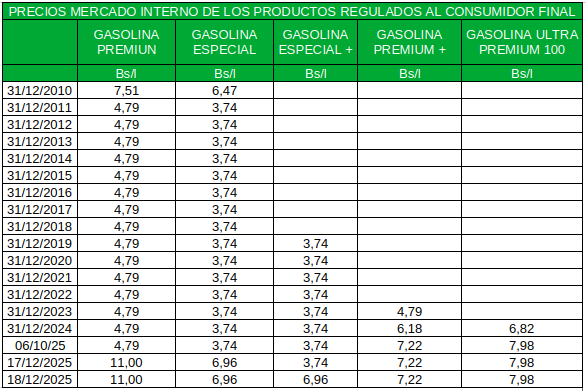
\includegraphics[width=0.9\textwidth]{Images/ANH.png}
	\vspace{0.2cm}
	
	% 3. La nota de fuente formateada según APA 7
	\begin{flushleft}
		\footnotesize \textit{Nota.} El gráfico muestra la tendencia histórica del costo del combustible. Tomado de \citep{anh_calidad_2024}.
	\end{flushleft}
\end{figure}

Asimismo, una combustión ineficiente asociada a combustibles de calidad variable puede influir en las lecturas de los sensores del vehículo, afectando la precisión de los sistemas de diagnóstico basados en OBD-II. Esto dificulta la interpretación adecuada de los parámetros del motor y limita la capacidad del usuario para evaluar el estado real de su vehículo.

En este escenario, surge una creciente preocupación sobre la eficiencia en el uso de la gasolina como fuente energética en el transporte, especialmente en vehículos que no cuentan con sistemas avanzados de monitoreo. La falta de herramientas accesibles que permitan analizar el consumo de combustible en tiempo real incrementa la incertidumbre del usuario respecto al rendimiento de su vehículo.

Por lo tanto, se plantea la necesidad de desarrollar un sistema que permita monitorear y analizar el consumo de combustible de manera precisa y en tiempo real, con el objetivo de contribuir a la optimización de la eficiencia energética del vehículo y brindar al usuario información confiable para la toma de decisiones \citep{lamby2026giro}.



\section{Justificación}

En el transporte urbano de La Paz, los vehiculos con sistemas de inyección electrónica operan sin herramientas que permitan conocer de manera precisa y continua el consumo real de gasolina durante su funcionamiento. En la práctica, la evaluación del consumo se realiza de forma empírica, sin información técnica que permita identificar ineficiencias en el uso del combustible.

La ausencia de sistemas de monitoreo del consumo dificulta el análisis del comportamiento del motor, tales tramos recorridos y modos de conducción. Esta situación limita la posibilidad de optimizar el desempeño del vehículo y detectar posibles fallas asociadas a un consumo anómalo de combustible El proyecto ayuda a tener un patrón o un control que indica si el vehículo consume mas gasolina de la que debe, considerando las condiciones en la ciudad de La Paz.

El desarrollo de un sistema permitirá generar información confiable sobre el comportamiento del motor. Esta información contribuirá a la mejora de la eficiencia operativa, al análisis técnico del consumo de combustible y al apoyo en procesos de mantenimiento y toma de decisiones técnicas.
\begin{itemize}
	\item \textbf{Justificación técnica:}
	El proyecto propone el desarrollo de un sistema de monitoreo del consumo de gasolina basado en la adquisición de parámetros del motor a través del puerto OBD-II y su procesamiento mediante un modelo físico-matemático del proceso de inyección de combustible. A diferencia de los métodos convencionales basados únicamente en mantenimiento correctivo o preventivo \citep{Reif2015}, la propuesta integra una plataforma telemétrica capaz de adquirir datos del vehículo, permitiendo el análisis casi en tiempo real del comportamiento del motor.
	
	\item \textbf{Justificación económica:}
	El acceso a información precisa y continua sobre el consumo de combustible permite a conductores y operadores de transporte optimizar el uso del vehículo, reduciendo gastos innecesarios asociados al consumo excesivo de gasolina. Asimismo, el sistema contribuye a la toma de decisiones relacionadas con el mantenimiento del motorizado y la planificación de rutas, generando un impacto económico positivo tanto para transportistas como para usuarios.
	
	\item \textbf{Justificación social:}
	El sistema propuesto aporta a la mejora de la eficiencia del transporte urbano y vehículos de uso particular, al promover un uso más responsable del combustible. Esto contribuye indirectamente a una mayor transparencia en el desempeño de los vehículos, a la concienciación sobre el consumo energético y a la mejora de la calidad del servicio de transporte en la ciudad de La Paz.
\end{itemize}

\section{Objetivos del proyecto}
\subsection{Objetivo General}
\begin{itemize}
	\item Desarrollar e implementar un sistema embebido capaz de adquirir datos en tiempo real desde el puerto de diagnóstico vehicular mediante el estándar OBD-II, con el fin de estimar el consumo instantáneo de combustible en vehículos a gasolina con inyección electrónica, generar un registro histórico de consumo y validar los resultados respecto a mediciones de referencia.
\end{itemize}

\subsection{Objetivos específicos}
\begin{itemize}
	\item Determinar los parámetros del sistema OBD-II disponibles, particularmente el flujo de aire del motor (MAF) y/o presión de aire del motor (MAP), las RPM y la velocidad del vehículo, con el fin de estimar el consumo de combustible mediante un modelo matemático basado en la relación aire-combustible.
	
	\item Desarrollar un modelo matemático para la estimación del consumo de combustible del transporte público de la ciudad de La Paz, utilizando parámetros obtenidos mediante el sistema OBD-II, basado en la relación aire--combustible del proceso de combustión.
	
	\item Adquirir y registrar datos del funcionamiento del motor mediante el sistema OBD-II, particularmente el flujo másico de aire (MAF) y/o presión de aire del motor (MAP), las revoluciones por minuto (RPM) y la velocidad del vehículo, para su posterior análisis en el modelo de estimación del consumo de combustible. Como se menciona en \citep{shaw2019fuel}, es posible estimar el consumo instantáneo de combustible utilizando datos obtenidos del vehículo mediante interfaces OBD-II.
	
	\item Diseñar un sistema embebido de adquisición de datos para la captura, el guardado y posterior procesamiento de estos, facilitando la validación del modelo matemático de consumo de combustible del transporte público de La Paz.
	
	\item Diseñar e implementar una plataforma telemétrica basada en arquitectura IoT para la adquisición de parámetros del motor a través de la interfaz OBD-II utilizando un módulo ESP32  conectado a un adaptador , permitiendo la transmisión de los datos mediante un protocolo de comunicación hacia un servidor local donde serán almacenados en una base de datos estructurada para su posterior análisis del consumo de combustible.
	
	\item Evaluar el sistema integral del transporte público de La Paz bajo condiciones reales, validando su precisión en la estimación del consumo de combustible y su contribución a la mejora de la eficiencia energética.
	
\end{itemize}

\section{Alcances y limites}
\subsection{Alcances}
El presente proyecto tiene como alcance el desarrollo de un sistema de monitoreo del 
consumo de combustible basado en la adquisición de datos a través del puerto OBD-II 
del vehículo, utilizando un microcontrolador ESP32C3 y un módulo de comunicación CAN.
El sistema tendrá los siguientes alcances:

\begin{itemize}
	\item Lectura de parámetros vehiculares en tiempo real, tales como revoluciones 
	del motor (RPM), velocidad del vehículo y otras variables disponibles mediante el 
	protocolo OBD-II, las cuales serán utilizadas para la estimación del consumo 
	de combustible.
	
	\item Procesamiento de los datos obtenidos con el fin de generar información 
	comprensible para el usuario, permitiendo evaluar el rendimiento del vehículo 
	en función de su consumo energético.
	
	\item Desarrollo de una interfaz de monitoreo accesible mediante una página web 
	generada por el propio ESP32, disponible a través de una dirección IP local, 
	que permitirá la visualización de los datos en tiempo real sin necesidad de 
	software adicional.
	
	\item Diseño, implementación y validación del sistema en condiciones reales de 
	funcionamiento, permitiendo verificar su desempeño en la estimación del consumo 
	de combustible.
\end{itemize}
\subsection{Limites}

La solución propuesta presenta ciertas limitaciones técnicas y de alcance que deben ser consideradas para una correcta interpretación de los resultados.

\begin{itemize}
	\item Una de las principales limitaciones está relacionada el tipo de combustible del vehículo.El desarrollo se enfoca exclusivamente a vehículos a gasolina con inyección electrónica, también no se enfoca a vehículos con diésel o con sistemas de combustible combinado, conocidos como vehículos \textit{bi-fuel}, los cuales pueden operar tanto con gasolina como con gas natural o GLP. Debido a que el comportamiento físico y energético de estos combustibles es diferente, el sistema propuesto se enfoca únicamente en vehículos que operan exclusivamente con gasolina, no siendo posible un control preciso del consumo en vehículos bi-fuel \citep{AFDC_BiFuelVehicles}.
	\item Asimismo, los vehículos de modelos antiguos que cuentan con sistemas de diagnóstico OBD-I presentan una limitación importante, ya que no permiten el acceso a información estandarizada del motor. Por esta razón, el sistema se encuentra limitado a vehículos que disponen de puerto OBD-II o sistemas de diagnóstico compatibles.
	\item En el contexto del transporte público en la ciudad de La Paz, la compatibilidad con sistemas de diagnóstico a bordo OBD-II se encuentra en vehiculos de fabricación relativamente reciente. En el presente trabajo se considerarán únicamente modelos que dispongan de esta tecnología, sin especificar marcas o versiones comerciales particulares.
	No obstante, el análisis experimental se limitará exclusivamente a unidades seleccionadas que cumplan con el requisito de compatibilidad OBD-II.
	\item Una de las limitaciones del presente estudio es la disponibilidad de
	vehículos para la realización de las pruebas experimentales. Al no disponer
	de acceso directo y permanente a unidades específicas como en el caso de los minibuses. Por esta razón, las pruebas experimentales podrán
	realizarse también en otros vehículos con características mecánicas
	similares que formen parte del parque automotor urbano y que
	cuenten con sistemas de inyección electrónica compatibles con la
	interfaz OBD-II.
	\item Adicionalmente, la precisión del sistema dependerá del estado mecánico del vehículo . En vehículos con alto kilometraje o desgaste significativo, los valores obtenidos pueden presentar variaciones respecto a los valores ideales.
\end{itemize}
\clearpage